
\documentclass[12pt]{article} 

%?? paths
\newcommand{\CiteMathPackage}{../../math} 
\newcommand{\CiteReference}{../reference.bib}

%?? packages 
\usepackage{setspace,geometry,fancyvrb,rotating} 
\usepackage{marginnote,datetime,enumitem} 
\usepackage{titlesec,indentfirst} 
\usepackage{amsmath,amsfonts,amssymb,amsthm,mathtools} 
\usepackage{threeparttable,booktabs,adjustbox} 
\usepackage{graphicx,epstopdf,float,soul,subfig} 
\usepackage[toc,page]{appendix} 
\usdate

%?? page setup 
\geometry{scale=0.8} 
\titleformat{\paragraph}[runin]{\itshape}{}{}{}[.] 
\titlelabel{\thetitle.\;} 
\setlength{\parindent}{10pt} 
\setlength{\parskip}{10pt} 
\usepackage{Alegreya} 
\usepackage[T1]{fontenc}
% \usepackage{fourier} % Favorite Font

%?? bibliography 
\usepackage{natbib,fancybox,url,xcolor} 
\definecolor{MyBlue}{rgb}{0,0.2,0.6} 
\definecolor{MyRed}{HTML}{D2042D}
\definecolor{MyGreen}{rgb}{0,0.4,0} 
\definecolor{MyPink}{HTML}{E50379} 
\definecolor{MyOrange}{HTML}{CC5500} 
\definecolor{MyPurple}{HTML}{BF40BF}
\newcommand{\highlightR}[1]{{\emph{\color{MyRed}{#1}}}} 
\newcommand{\highlightB}[1]{{\emph{\color{MyBlue}{#1}}}} 
\newcommand{\highlightP}[1]{{\emph{\color{MyPink}{#1}}}} 
\newcommand{\highlightO}[1]{{\emph{\color{MyOrange}{#1}}}}
\newcommand{\highlightPP}[1]{{\emph{\color{MyPurple}{#1}}}}
\usepackage[bookmarks=true,bookmarksnumbered=true,colorlinks=true,linkcolor=MyGreen,citecolor=MyGreen,filecolor=MyBlue,urlcolor=MyGreen]{hyperref} 
\bibliographystyle{econ}

%?? math and theorem environment 
\theoremstyle{definition} 
\newtheorem{assumption}{Assumption} 
\newtheorem{definition}{Definition} 
\newtheorem{theorem}{Theorem} 
\newtheorem{proposition}{Proposition} 
\newtheorem{lemma}{Lemma} 
\newtheorem{example}{Example} 
\newtheorem{corollary}[theorem]{Corollary} 
\usepackage{mathtools} 
\usepackage{\CiteMathPackage}

\begin{document} 

%??%??%??%??%??%??%??%??%??%??%??%??%??%??%??%??%??%??%??%??%??%?? 
%?? title 
%??%??%??%??%??%??%??%??%??%??%??%??%??%??%??%??%??%??%??%??%??%??

\title{\bf The U-Shapes of Occupational Mobility, Review of Economic Studies, 2015} 
\author{Wenzhi Wang \thanks{This note is written in my pre-doc period at the University of Chicago Booth School of Business.} } 
\date{\today} 
\maketitle 

\citet{groesUShapesOccupationalMobility2015}

\section{Introduction}

Danish employers report that every year close to a one fifth of their workers change occupations (e.g. technician, engineer, manager). Similar levels of occupational mobility are reported for the U.S. Moreover, these gross flows are much larger than the net flows that are needed to account for the changing sizes of occupations. What induces workers to undertake these occupational changes? The answer to this question seems especially interesting because occupational choices and wages are closely related. First, the differences in average occupational wages are substantial and persistent. Secondly, it has recently been argued that the returns to occupational tenure are nearly as large as the returns to labour market experience and much larger than the returns to firm or industry tenure. Thus, understanding workers' occupational choices is important for understanding the allocation of the labour force across productive activities, for interpreting earning patterns, for measuring the returns to human capital accumulation, and for assessing the effects of various policies affecting sorting of workers across occupations. Since occupational choices are endogenous, the outcome of such analysis will depend on the theory used to account for selection of workers across occupations. Although there exist a number of theories of occupational choice, it remains an open empirical question which selection process is consistent with the data.

This article contributes to our understanding of selection in occupational choices by looking at occupational mobility data in a novel way. Using administrative data on 100\% of the Danish workforce we provide new direct evidence on patterns of worker mobility across occupations. This evidence conflicts with several existing theories that are often used to account for the endogeneity in occupational choice, but we can show analytically that the patterns are explained consistently within a theory of vertical occupational mobility combined with learning about worker ability.

\highlightP{We document that for most occupations, mobility is U-shaped and directional}: it is both the low wage and high wage workers within an occupation who have a particularly large probability of leaving that occupation, while the lowest probability of leaving is associated with the medium wage workers within the occupation. More than three-quarters of the labour force are employed in occupations exhibiting this pattern. Altough switching probabilities are particularly high at both ends of the wage spectrum within an occupation, the direction of sorting is very different for high and low wage earners. Those earning low wages relative to other workers relative to other workers in the same occupation tend to leave for new occupations that on average pay less to their workforce than the old occupation, whereas those with high relative wages in their occupation tend to leave for occupations that on average pay more to their workforce. These patterns remain whether we focus on workers who stay with the same firm or on those who switch firms, and across various ways of defining occupations. The U-shaped mobility pattern is pre-dominant except for occupations with steeply rising (declining) productivity, from which mainly the lower (higher) paid workers tend to leave.

We are able to document these patterns because the data allow us to compare the behaviour of different workers in the same occupation. Such analysis has been missing in the literature partly because most longitudinal data sets that have traditionally been analyzed feature only panels of a few thousand workers, and with around three hundred occupations, an analysis on a per occupation basis was not feasible. This new look at the data has at least two important direct implications:
\begin{itemize}[topsep=0pt, leftmargin=20pt, itemsep=0pt]
	\setlength{\parskip}{10pt} 
	\item First, selection is not just one-sided. In particular, the well-documented wage growth with tenure in an occupation is not just due to low wage earners leaving and high wage earners staying. In fact, a large number of high wage earners are leaving their occupations as well, and models generating the wage implications based on worker selection need to take this into account.
	\item Secondly, occupations with strong productivity growth nevertheless shed a large fraction of their workforce, a stark feature of the data not featured by the commonly used models.
\end{itemize}

A number of prominent models of occupational choice feature counterfactual one-sided selection, typically with relatively low wage earners leaving the occupation whereas high wage earners stay. One popular class of such models is based on \highlightR{horizontal sorting due to match-specific shocks}. This work is based on the idea that occupations are identical (not different with respect to skill requirements), but workers find out the quality of their idiosyncratic match with an occupation over time. Horizontal re-sorting occurs when workers realize that their match-specific productivity is low and abandon the match in favor of (and search for) a better one. Thus, the model predicts that workers with low wages (low quality matches) leave the occupation, and their next occupational choice is a rando draw. Both predictions do not match up with our findings in the data. 

Similarly, island economy models based on human capital extensions of \citet{lucasEquilibriumSearchUnemployment1974} typically predict that it is the low human capital and hence, low wage workers who are the first to switch if occupational demand declines since high human capital workers have more incentive to wait for the conditions to improve. If occupational demand rises, no one leaves the occupation. The wage a switcher obtains in the new occupation is independent of her relative wage in the previous occupation. Once again, these implications do not match up with the patterns we find in the data. 

Nevertheless, we show theoretically that selection based on vertical sorting where more able workers are matched with more productive occupations does account well for all of the qualitative empirical patterns. High-ability workers within an occupation tend to earn high wages, and changes to their perceived ability can lift them beyond the threshold where it is optimal to move to a more skill-intensive occupation, inducing (predominantly) upward mobility. Workers whose perceived ability is such that they obtain wages close to the middle of the occupational wage distribution are less likely to update their beliefs sufficiently to warrant a move to a new occupation, so their mobility is lower. Low-ability workers within an occupation tend to earn lower wages and changes to their perceived ability might induce them to move to an occupation with lower skill-requirements, inducing (predominantly) downward mobility. Although there are many reasons why perceived ability may be changing (some are discussed below), one plausible reason is that workers' ability gets revealed only slowly over time through observations of labour market performance, as formalized in the decision-theoretic work of Gibbons and Waldman (1999) that was successfully used to understand mobility and promotion dynamics within firms. Our model is an extension of this framework to a general equilibrium setting where wages are set in competition for workers. This is similar to \citet{papageorgiouLearningYourComparative2014}, although we abstract from a number of elements (search frictions, differential speed of learning) to be able to provide a clear and easily comprehensible insight on sorting across many occupations.

In addition to accounting for the qualitative U-shaped mobility patterns and the direction of switching, this theory also has secondary implications that conform well with the data. Considering occupations with roughly constant productivities, the theory predicts that workers who switch to occupations with higher average wages see faster wage growth than workers who stay, who, in turn, see faster wage growth than workers who move to occupations with lower average wages. In terms of wage levels, those who switch to an occupation with higher average wages do better than those who remain in the old occupation, but worse than those who already work in the new occupation. The opposite holds for workers that move occupations with lower average wages. Older workers switch occupation less frequently, and their wage distribution is more dispersed than that of younger workers. \highlightP{Finally, the equilibrium nature of the model implies that occupations with sharply increasing productivity will retain their high earners but shed their low earners, and the opposite holds for occupations with a substantial decline in productivity.}

Therefore, vertical re-sorting as a consequence of changes in perceived ability seems a promising avenue to account and control for endogenous occupational mobility. This view of labour market has a long tradition, even though in the context of occupational mobility horizontal sorting and match-specific shocks have arguably received more attention. Vertical sorting is a basic feature of the famous Roy (1951) specification with absolute advantage, and its combination with learning about workers' permanent ability hs been explored in many settings. We discuss the similarities and the differences from the Roy (1951) model explicitly. \highlightP{Then main distinguishing features arises in the presence of occupational productivity shocks, where decision-theoretic models imply that a rising occupational productivity will make the occupation more attractive for all workers, whereas in our equilibrium model it becomes more attractive only for the more productive workers who compete with and drive out the less able workers.} In contrast to other equilibrium models, the main advantage of our formulation is its simplicity, which allows us to easily handle many occupations which is necessary to derive many of the important results. In line with all the work cited in this paragraph, we abstract from an explicit notion of firms. Our main reason is that in the data the pattern of occupational switching is similar for workers who stay with the same firm as for those who switch firms.

The main message of this article concerns the nature of occupational selection. Selection at the bottom of the within-occupation wage spectrum has long been emphasized and is very intuitive: Low wages are are indication that a person should be doing something else, who therefore has a tendency to leave the occupation. If that were the only source of selection, in the cross-section wages would increase with occupational tenure simply because only high wage earners stay. In contrast, we highlight that selection is equally strong at the top of the within-occupation wage spectrum. This suggests that high wages are not a sign that a person is particularly well matched his/her current occupation: in a world with vertically differentiated occupations we show that this is rather a sign of overqualification that induces workers to seek more suitable types of worker. If this is the case, the dominant direction of mobility of high earners should be different from that of low earners, which is consistent with the pattern we document in the data. 

Of course, we do not think that the simple vertical sorting mechanism that we propose accounts for the full extent of occupational mobility. In the Conclusion, we discuss the broader research agenda, and the challenges to the empirical assessment of the exact quantitative implications of the patterns presented in this article. \highlightR{Both vertical and horizontal moves likely arise in the labour market, i.e. some occupations are considered better than others whereas some are just different and people switch along both of these dimensions} (e.g. in a complementary work \citet{papageorgiouLearningYourComparative2014} finds evidence of substantial horizontal worker sorting across three broad occupational categories based on the comparative advantage). And among those occupations that can be ranked as better or worse, the ranking might change over time. Therefore, it is likely that match-specific components and the volatility of productivities of occupations or of the demands for their services are responsible for a non-trivial share of mobility. \highlightR{An important part of a future agenda is to identify which occupations form vertical hierarchies to identify the costs of switching within and across hierarchies.} Our analysis suggests that many of the occupational switches do arise within hierarchies. Therefore, we do think that the mechanism we emphasize should be an important part of any comprehensive theory of occupational mobility.

\section{The U-Shapes of Occupational Mobility: Evidence}

\subsection{Data}

{The hourly wage variable is calculated as the sum of total labour market income and mandatory pension fund payments of the job held in the last week in November of a given year divided by the total number of hours worked in the job held in November of that year.} 

\subsection{U-Shapes in the Probability of Occupational Switching}

For each worker that we observe in a given year of our sample, we compare his/her wage to the wages of the other workers in the same occupation in the same year. This gives us this worker's rank in the wage distribution of his/her occupation. That is, it gives the fraction of other workers in the same occupation that earn lower wages than him/her this year. We plot the probability of switching to a new occupation in the following year against this rank. 

Figure \ref{groesUShapesOccupationalMobility2015_fig1}(a) is a non-parametric plot (from a kernel smoothed local linear regression with bandwidth of $5$ percentiles) of the probability of switching out of an occupation as a function of a worker's position in the wage distribution in that occupation in a given year.

\begin{figure}[H]
    \noindent\caption{Non-parametric plot of probability of switching occupation by worker's percentile in the relevant wage distribution}
    \begin{center}
        \resizebox{0.7\textwidth}{!}{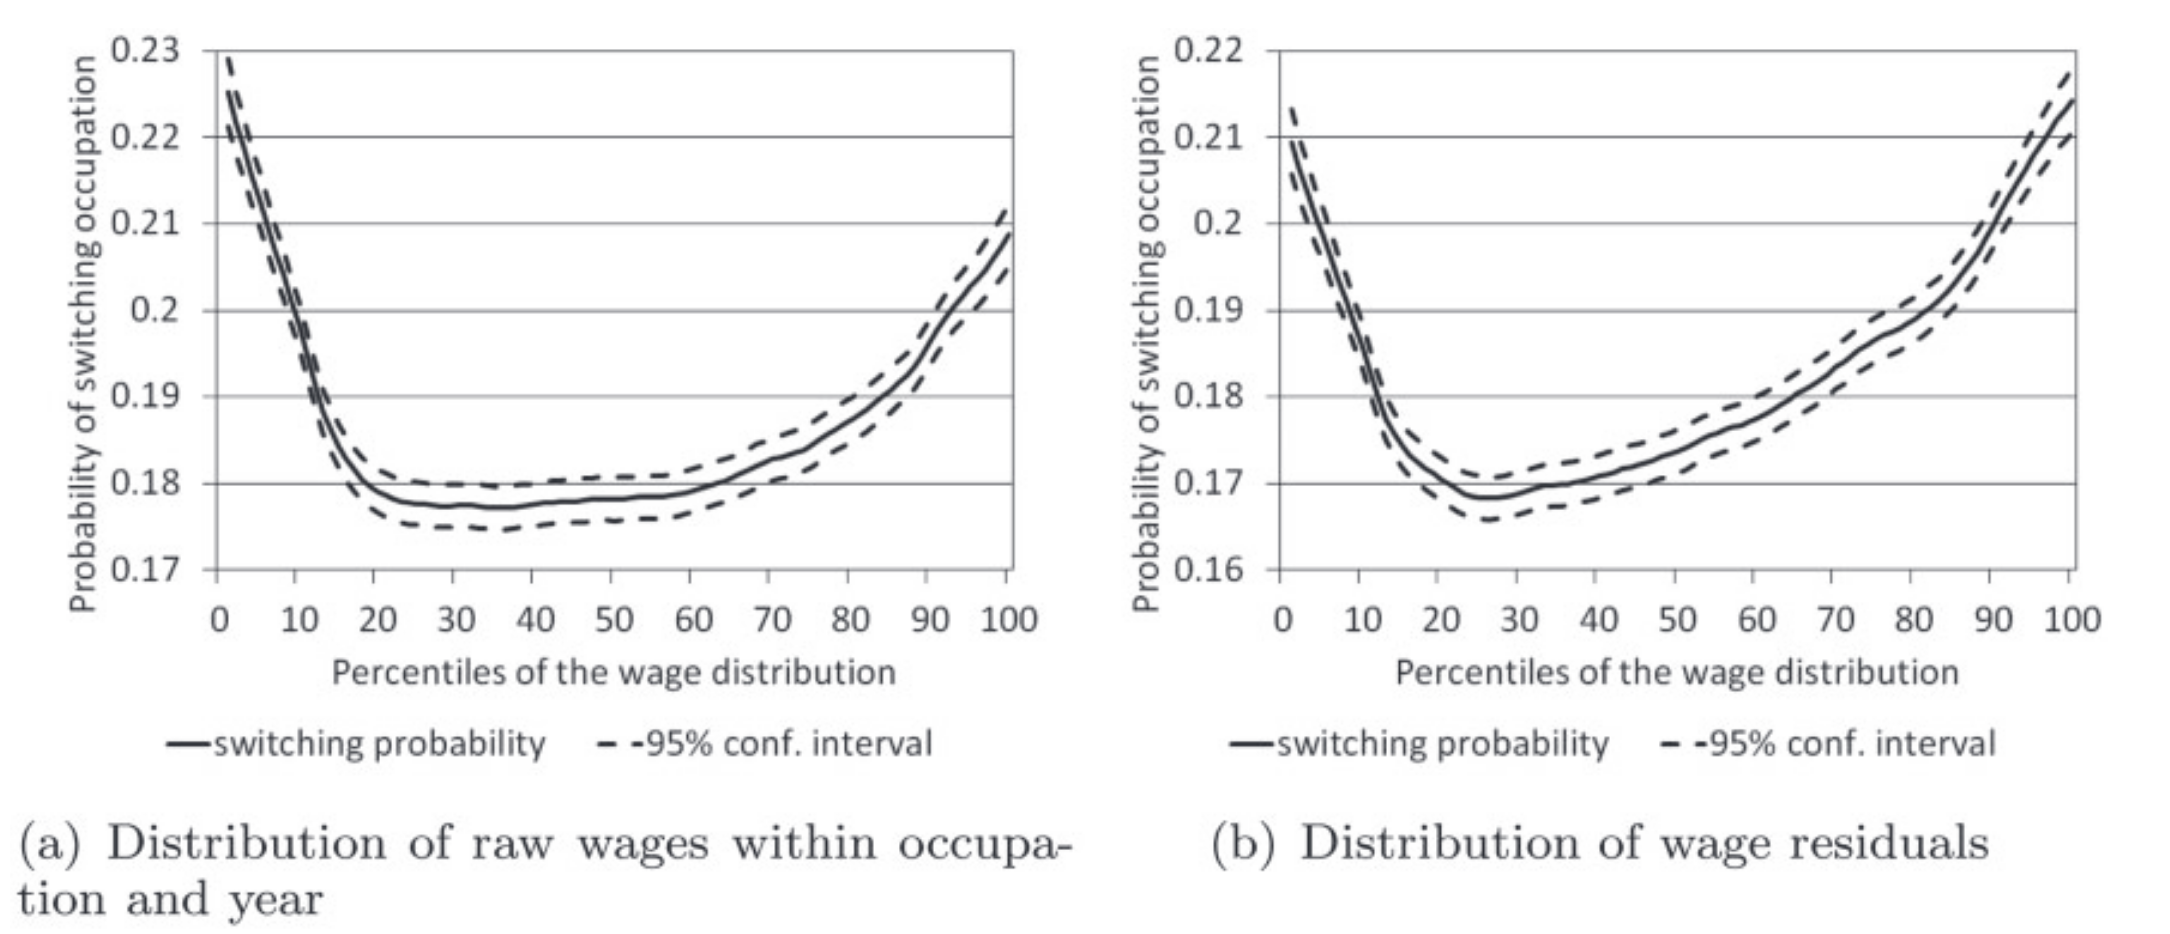
\includegraphics{groesUShapesOccupationalMobility2015_fig1.png}}
        \label{groesUShapesOccupationalMobility2015_fig1}
    \end{center}
\end{figure}

Figure \ref{groesUShapesOccupationalMobility2015_fig1}(a) is based on raw wage data. Figure \ref{groesUShapesOccupationalMobility2015_fig1}(b) indicates that we also observe a U-shaped pattern of occupational mobility in the position of the worker in the distribution of residual wages in his/her occupation in a given year. We generate residual wages by estimating a standard reduced-form wage regression 
\begin{equation}
    \label{groesUShapesOccupationalMobility2015_eq1}
    \ln\of{w_{ijt}} = X_{ijt} \b + \e_{ijt},
\end{equation}
where $w_{ijt}$ is real hourly wage of individual $i$ working in occupation $j$ in period $t$ and $\e_{ijt}$ is the residual. The explanatory variables in $X$ include calendar year dummies, third degree polynomials in general experience, occupational tenure, industry tenure, a second-degree polynomial in firm tenure, the sequence number of occupational spell, education, marital status, union membership, and lagged regional unemployment rates. These wage regressions are estimated separately for each occupation.

\subsection{U-Shapes in the Direction of Occupational Switching}

In this section, we document another prominent feature of the data: conditional on chaning occupation, workers with higher (lower) relative wages within their occupation tend to switch to occupations with higher (lower) average wages than the average wage in their current occupation. We first find the average wage of all occupations in a given year to determine the ranking between occupations. Similarly to our analysis of probability of occupational switching, we rank occupations based on their raw wages or residual wages adjusted for worker characteristics. To obtain the ranking based on raw wages, we find the average real wage of all full-time private-sector workers in a given occupation in a given year. To obtain the ranking based on residual wages, we use our selected sample to run a similar wage regression as in equation (\ref{groesUShapesOccupationalMobility2015_eq1}) for each occupation where we include time dummies in the regression (without the intercept). We interpret the coefficients on these time dummies as the average occupational wage in a given year, adjusted for human capital accumulation of workers in the occupation as well as other worker characteristics such as education, regional dummies, and marital status.

\begin{figure}[H]
    \noindent\caption{Non-parametric plot of direction of occupational mobility, conditional on switching occupation, by worker's percentile in the relevant wage distribution before the switch}
    \begin{center}
        \resizebox{0.7\textwidth}{!}{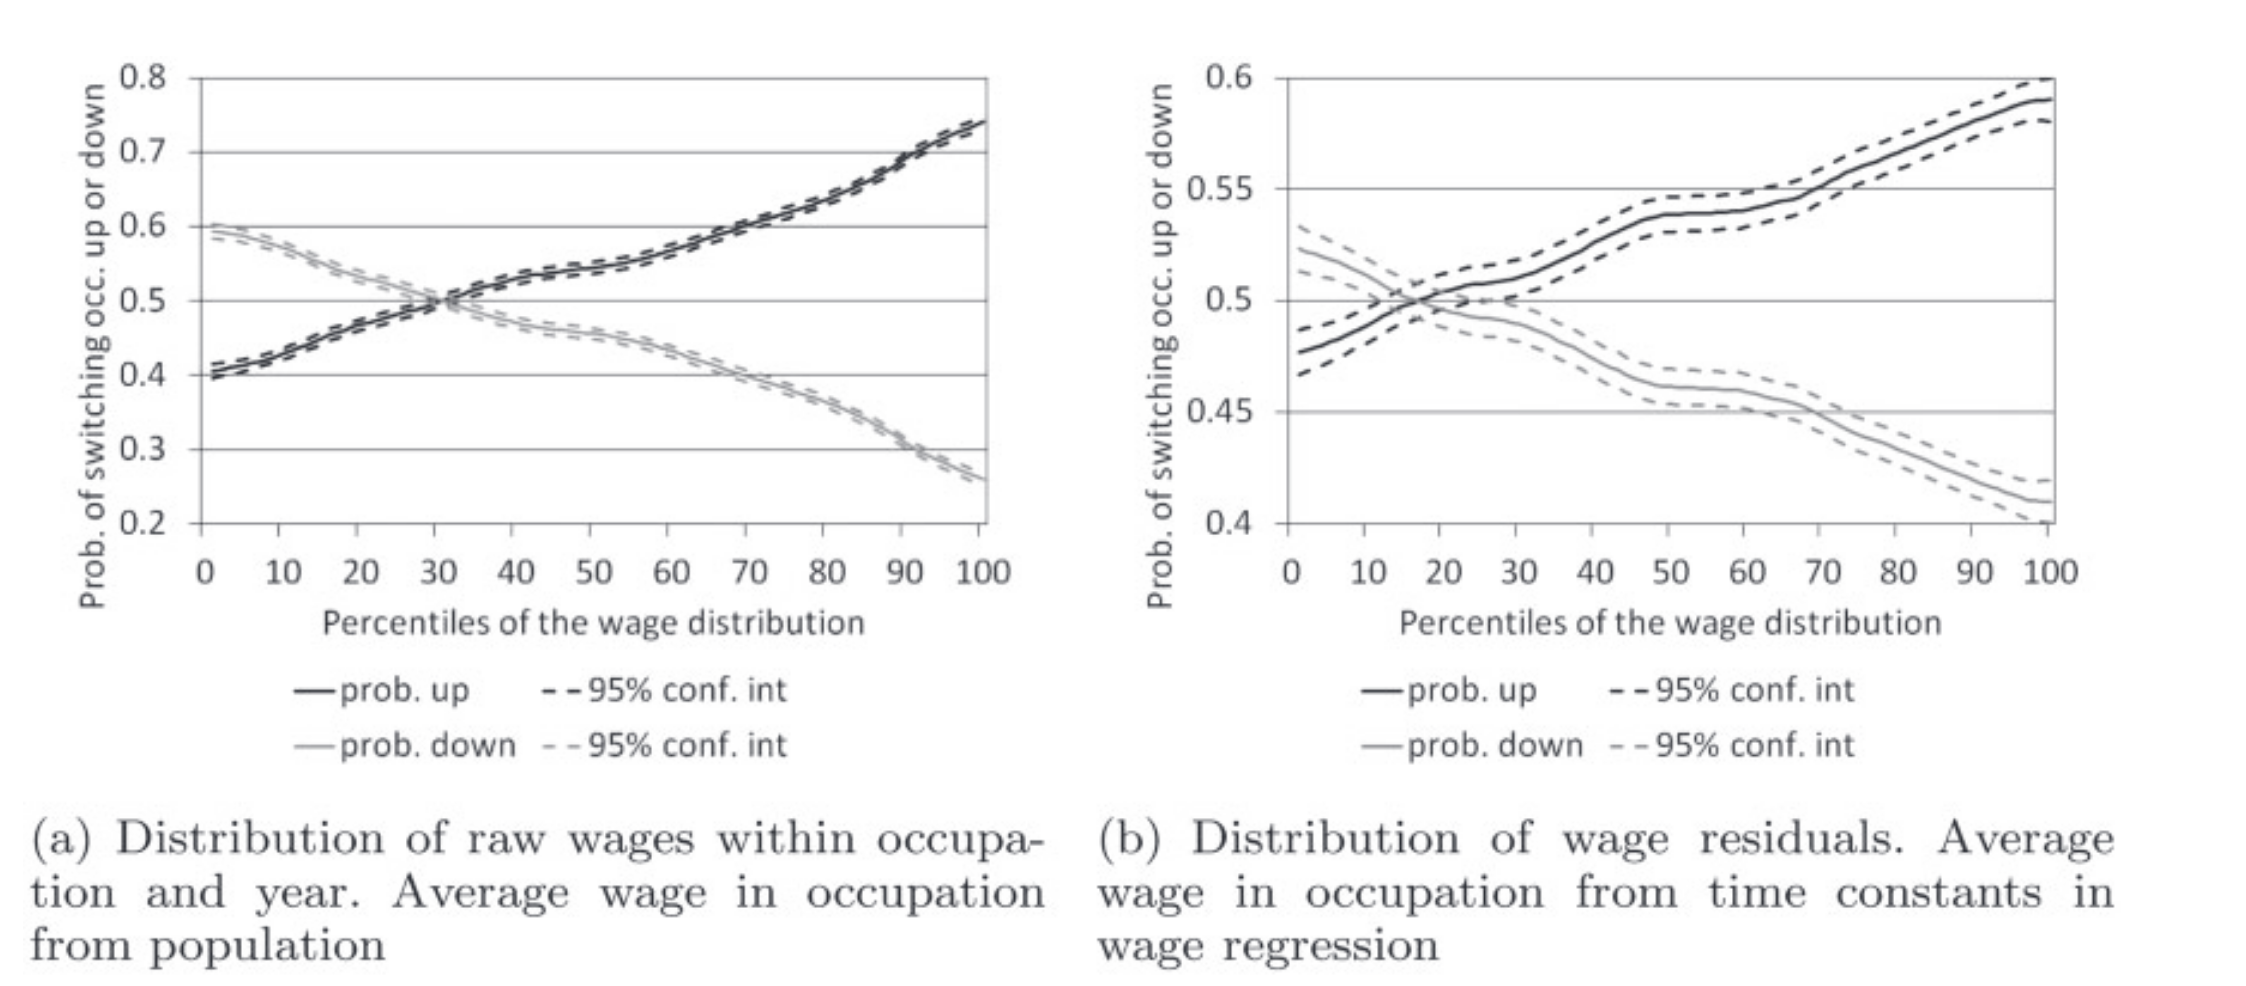
\includegraphics{groesUShapesOccupationalMobility2015_fig3.png}}
        \label{groesUShapesOccupationalMobility2015_fig3}
    \end{center}
\end{figure}

Figure \ref{groesUShapesOccupationalMobility2015_fig3}(a) plots the probability of switching to an occupation with a higher or lower average wage as a function of the worker's position in the wage distribution of the occupation of the occupation he or she is leaving. \highlightPP{The sample on which the figure is based consists of all workers who switched occupation in a given year and occupations are ranked based on the raw average wages.} Figure \ref{groesUShapesOccupationalMobility2015_fig3}(b) presents corresponding evidence when occupations are ranked based on residual wages and the direction of occupational mobility is plotted against the percentile in the distribution of residual wages within an occupation the worker is switching from. 

The evidence contained in these figures suggests that, conditional on switching occupations, the higher relative wage a person has in his/her occupation before the switch, the higher is the probability that he/she will switch to an occupation with a higher average wage. Similarly, the lower relative wage a worker has in his/her occupation before the switch, the higher is the probability that he/she will switch to an occupation with a lower average wage than in the occupation he/she switches from.

\subsection{Discussion of Empirical Evidence}

\subsubsection{Magnitudes of changes in occupational ranks}

\subsubsection{U-shapes of occupational mobility within and between firms}

\subsubsection{The U-shapes of occupational mobility: females}

\subsubsection{Alternative occupational classifications}

\subsubsection{The effects of measurement error}

\subsubsection{Focus on occupational mobility}

\subsubsection{Summary}

\section{The U-Shapes of Occupational Mobility: Theory}

In this section, we present a model of vertical sorting, where gross mobility arises since workers initially have only limited information about their ability and learn about it over time. In the model it is efficient that workers of higher ability work in the occupations where ability is most valued. If a worker learns that he/she is much better (or worse) than expected, he/she adjusts (has to adjust) to an occupation commensurate with his/her ability.

We show that the combination of learning and sorting is sufficient to generate the qualitative patterns we find in the data. TO highlight the basic impact of these two features, we abstract from other factors such as human capital accumulation and costs of occupational switching. We discuss in the Online Appendix how these features can be integrated. They do not offset the qualitative implications of sorting, but we discuss them because we expect them to be important for any quantitative assessment of the theory. Finally, we consider the validity of some secondary implications of the theory.

\subsection{The Model}

\subsubsection{Workers}

Workers choose employment in different occupations over time. Time is discrete and runs forever. Each period a unit measure of workers enters the labour market. The index for an individual worker will be $i$ throughout. Each worker is in the labour force for $T$ periods. Workers are risk-neutral and discount the future with a common discount factor $\b$. Each worker has an innate ability level $a_i$, i.e., drawn at the beginning of his life from a normal distribution with mean $\mu_a$ and variance $\s_a^2$. For the baseline model without human capital accumulation, we assume that this ability remains constant throughout a worker's life. The amount of output that a worker can produce depends on his/her ability. In particular, he/she produces 
\begin{equation}
    \label{groesUShapesOccupationalMobility2015_eq2}
    X_{i,t} = a_{i} + \ve_{i,t}
\end{equation}
in a given period $t$ of his/her life, where $\ve_{i,t}$ is a normally distributed noise term with mean zero and variance $\s_{\ve}^{2}$. Workers do not know their ability (and neither do firms), but workers observe the output they produce. We assume that the worker observes an initial draw after finishing school, i.e. before entering the labour market.

Over time, workers learn about their true ability, Let $\f_a = 1 / \s_a^2$ and $\f_{\ve} = 1 / \s_{\ve}^2$ denote the precision for each distribution, which is defined as the inverse of the variance. Define the cumulative precision of a worker at the beginning of his/her $t$th year in the labour market as $\f_t \coloneqq \f_a + t \f_{\ve}$. Initially, every worker only knows that his/her ability is distributed with mean $A_0 = \mu_0$ and precision $\f_0 = \f_a$. Standard results on updating of normal distributions establish that his/her belief at the beginning of every period $t > 0$ of his/her life is normally distributed with mean $A_{i,t}$ and precision $\f_t$, where the mean is determined successively by the output realizations that he/she observes. After observing some output realization $X_{i,t}$ the new mean is given by the precision-weighted average of the prior mean and the output observation:
\begin{equation}
    \label{groesUShapesOccupationalMobility2015_eq3}
    A_{i, t+1} = \frac{\f_t}{\f_{t+1}} A_{i,t} + \frac{\f_{\ve}}{\f_{t+1}} X_{i,t}.
\end{equation}
From the point of view of the individual, this evolution of the posterior is a martingale with decreasing variance: the weight on the prior increases the more observations have already been observed in the past, i.e. the higher is $t$. Correspondingly, the weight on the most recent observation decreases with years in the labour market. For all practical purposes, equation (\ref{groesUShapesOccupationalMobility2015_eq3}) can be interpreted as some exogenous change in workers ability, even though the learning interpretation appears to be particularly natural. In the following, we will refer to $A_{i, t+1}$ as the expected ability or simply as the belief, and drop the person-identifier $i$ and/or the time identifier $t$ when there is no danger of confusion.

For completeness, we define the following two distributions. First, let $G_{t}\of{A_{t+1} \mid A_t}$ denote the distribution of next period's belief for a worker with current belief $A_t$. It is normal with mean $A_t$. In particular, its density $g_t$ is single-peaked and symmetric around its peak at $A_t$, and shifting the prior mean $A_t$ simply shifts the entire distribution about the posterior horizontally in the sense that $g_{t}\of{A_{t+1} \mid A_t} = g_{t}\of{A_{t+1}+\d \mid A_t+\d}$ for any $\d$. This is all we need for most proofs. We call the latter property lateral adjustment. Secondly, the cross-sectional $F_t\of{A}$ of beliefs among workers that start the $t$ period of their working life can be computed from equation (\ref{groesUShapesOccupationalMobility2015_eq3}) and is independent of any choices that agents make. Therefore, the measure of agents with belief below $A$ across all cohorts at any point in time, $F\of{A} = \sum_{t=1}^{T} F_{t}\of{A}$, can be computed prior to any analysis of occupational choice. This simplifies the specification of an equilibrium.

\subsubsection{Occupations}

There are a finite number of occupations, indexed by $k \in \bc{0, 1, \ldots, K}$, each with some fixed measure $\g_k$ of available jobs. We treat the number of jobs as exogenous in this exposition, yet the Online Appendix OA16 discusses how endogenous entry can be accommodated (limited entry and associated competition among workers for scarce jobs will be most important in Section 4 to explain the mobility patterns when occupational productivities change).

Each unit of good (or service) i.e. produced sells in the market at some exogenously given price $P_k$. Therefore, worker $i$ employed in a job of type $k$ generates revenue 
\begin{equation}
    \label{groesUShapesOccupationalMobility2015_eq4}
    R_{ki} = P_k X_i.
\end{equation}
Equivalently, we can interpret $P_k$ as the productivity in terms of efficiency units of the labour (at a common sale price of unity). We rank occupations in order of increasing productivity such that $P_K > \ldots > P_{k} > \ldots > P_0 = 0$. Therefore, any given worker produces more in a higher ranked occupation. One can view the lowest ranked occupation as home production. An output signal is observable even in home production, and home production is available to everybody (more jobs than population size: $\g_0 \geq T$). All other jobs are assumed to be scarce (less jobs than workers with  positive ability: $\sum_{k=1}^{K} \g_k < T - F\of{0}$).

\subsubsection{Wages}

We consider a competitive economy without matching frictions. The only frictions are information frictions in the sense that workers' actual abilities are not known. There are (at least) two ways to think about wage setting in our economy. Wages might be output contingent contracts $w\of{X}$ that specify different wages based on the particular output that is realized. If a firm wants to obtain profits $\Pi_k$ it can simply offer the wage contract 
\begin{equation}
    \label{groesUShapesOccupationalMobility2015_eq5}
    w_k\of{X} = P_k X - \Pi_k 
\end{equation}
to any worker who is willing to take this contract. Since workers are risk-neutral, they choose the occupation with the highest expected wage. Therefore, it is not necessary that the firm has as much as information as the workers, since workers would self-select. The relevant sorting criterion for risk-neutral workers is their expected wage given their belief $A$ about their mean ability:
\begin{equation}
    \label{groesUShapesOccupationalMobility2015_eq6}
    W_{k}\of{A} = P_k A - \Pi_k.
\end{equation}
Alternatively, if the firm has the same information as the worker it can directly pay expected wages according to equation (\ref{groesUShapesOccupationalMobility2015_eq6}). In this case the firm absorbs all the risk. It would need to have the same information as the worker because otherwise it might attract workers with low expected abilities who try to get a high pay. Given risk-neutrality, whether firms or workers face the output risk does not affect the occupational choices by workers because in either case workers only care about expected wages (given by equation (\ref{groesUShapesOccupationalMobility2015_eq6})), but observed wages differ according to the specification and could potentially lead to different assessments of observed wage patterns. We will show our main qualitative results under both wage setting regimes. In fact, firms might pay workers according to some weighted average of equations (\ref{groesUShapesOccupationalMobility2015_eq5}) and (\ref{groesUShapesOccupationalMobility2015_eq6}) to provide both incentives for self-selection as well as insurance to workers, and our arguments can easily be extended to show that our main propositions hold for any such convex combination.

\subsubsection{Equilibrium}

We are considering a standard stationary competitive equilibrium in this matching market between occupations and workers. As market prices one can use either profits or wages, as one determines the other via equation (\ref{groesUShapesOccupationalMobility2015_eq5}) (or equation (\ref{groesUShapesOccupationalMobility2015_eq6})). It is notationally more convenient to focus on the profits. Stationary means that the entrepreneurs' profits $\Pi = \bp{\Pi_1, \Pi_2, \ldots, \Pi_K}$ and the associated wage offers are constant over time. The tractability of the baseline model arises from the fact that every period workers can costlessly re-optimize, and therefore, the sequence of decisions that maximize their lifetime income coincides to the sequence of decisions that maximizes their payoff in each period. Since the cross-sectional distribution of beliefs $F\of{A}$ remain constant, we can use standard tools for the analysis of static matching models. In particular, a worker will work in occupation $k$ rather than $k-1$ if the expected wage is higher: $P_k A - \Pi_k \geq P_{k-1} A - \Pi_{k-1}$. There is exactly one level of expected ability, call it $B_k$, at which this holds at equality:
\begin{equation}
    \label{groesUShapesOccupationalMobility2015_eq7}
    B_{k} \coloneqq \frac{\Pi_{k} - \Pi_{k-1}}{P_{k} - P_{k-1}}, \text{ for } k \in \bc{1, \ldots, K}.
\end{equation}
Therefore, workers optimally choose to work in occupation $k$ if their expected ability is within the interval $[B_k, B_{k+1})$, where we define $B_0 \equiv - \infty$ and $B_{K+1} \equiv \infty$. Market clearing then means that the number of workers $F\of{B_{k+1}} - F\of{B_k}$ that would like to work in occupation $k$ coincides with the number of jobs $\g_k$ available in this occupation:
\begin{equation}
    \label{groesUShapesOccupationalMobility2015_eq8}
    \g_k = F\of{B_{k+1}} - F\of{B_k}, \text{ for } k \in \bc{1, \ldots, K}.
\end{equation}
The system (\ref{groesUShapesOccupationalMobility2015_eq7}) and (\ref{groesUShapesOccupationalMobility2015_eq8}) can easily be solved recursively: Summing equation (\ref{groesUShapesOccupationalMobility2015_eq8}) across all $k$ and noting that $F\of{B_{K+1}}$ equals the total population $T$, we get $\sum_{k} \g_k = T - F\of{B_1}$ which determines $B_1$. Then successive application of equation (\ref{groesUShapesOccupationalMobility2015_eq8}) yields the remaining cut-off levels $\bp{B_2, \ldots, B_K}$. Since zero productivity in the lowest occupation implies zero profit, (\ref{groesUShapesOccupationalMobility2015_eq7}) then delivers the profits of the firms in the various occupations $\bp{\Pi_1, \ldots, \Pi_K}$. To sum up:

\begin{definition}
    An equilibrium is a vector of profits $\bds{\Pi} = \bp{\Pi_0, \ldots, \Pi_K}$ with $\Pi_0 = 0$ and a vector of optimal worker cut-off level $\bp{B_1, B_2, \ldots, B_K}$ such that equations (\ref{groesUShapesOccupationalMobility2015_eq7}) and (\ref{groesUShapesOccupationalMobility2015_eq8}) hold.
\end{definition}

\subsection{Analysis: shape and direction of occupational mobility}












\bibliography{\CiteReference} 

\end{document}